% This file is part of BenchExec, a framework for reliable benchmarking:
% https://github.com/sosy-lab/benchexec
%
% SPDX-FileCopyrightText: 2007-2020 Dirk Beyer <https://www.sosy-lab.org>
%
% SPDX-License-Identifier: CC-BY-4.0

\documentclass[tikz, border=3mm, convert=pdf2svg]{standalone}
\usetikzlibrary{arrows}
\usetikzlibrary{calc}
\usetikzlibrary{positioning}

\begin{document}
  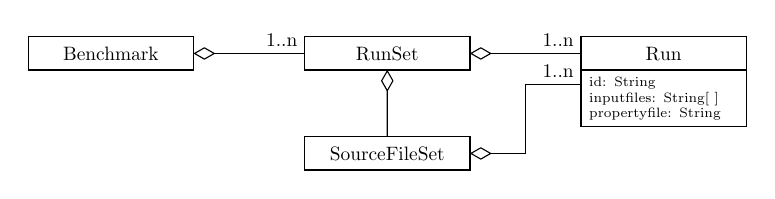
\begin{tikzpicture} [
        scale = 0.7,
        transform shape,
        node distance = 2cm,
        every node/.style = {
          align = center,
          %font = \footnotesize,
        },
        aggregation/.style = {
          draw,
          open diamond-,
        },
        umlbox/.style = {
          draw,
          minimum width = 3cm,
          minimum height = 0.6cm,          
        }
      ]

    % textboxes
    \node [umlbox] (Benchmark) {Benchmark};
    \node [umlbox, right = of Benchmark] (RunSet) {RunSet};
    \node [umlbox, right = of RunSet] (Run) {Run};
    \node [umlbox, below = 0cm of Run, align=left, font=\scriptsize, text width = 2.7cm] (desc) {id: String\\inputfiles: String[\ ]\\propertyfile: String};
    \node [umlbox, below = 1.2cm of RunSet] (SourceFileSet) {SourceFileSet};

    \draw[aggregation] (Benchmark) -- (RunSet.west) coordinate [label=135:{1..n}];
    \draw[aggregation] (RunSet) -- (SourceFileSet);
    \draw[aggregation] (RunSet) -- (Run.west) coordinate [label=135:{1..n}];
    \draw[aggregation] (SourceFileSet.east) -| ($(SourceFileSet.east)!.5!(desc.170)$) |- (desc.170) coordinate [label=135:{1..n}];
  \end{tikzpicture}
\end{document}
